\documentclass[border=3pt,tikz]{standalone}
\usepackage{amsmath}
\usetikzlibrary{calc}
\usetikzlibrary{arrows.meta} 
\tikzset{
  quadratic/.style={
    to path={
      (\tikztostart) .. controls
      ($#1!1/3!(\tikztostart)$) and ($#1!1/3!(\tikztotarget)$)
      .. (\tikztotarget)
    }
  }
}
% for arrow size
\begin{document}
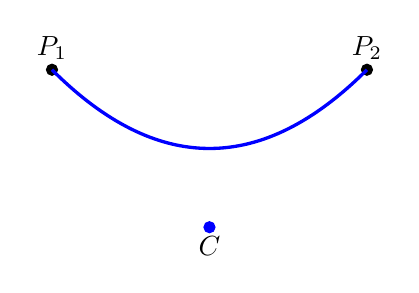
\begin{tikzpicture}[scale=1.0]
\filldraw [black] (-2, 2) circle (2pt) node[anchor=south] {$P_1$};;
\filldraw [black] (2, 2) circle (2pt) node[anchor=south] {$P_2$};
\filldraw [blue] (0,0) circle (2pt)node[anchor=north, black] {$C$};
\draw[blue,very thick] (-2, 2) to[quadratic={(0, 0)}] (2, 2);
\end{tikzpicture}
\end{document}